

\setcounter{section}{3}
\section{Hardware Design}
\bigskip
\subsection{System Design}

\pagebreak
\subsection{Communication Protocol}
\textbf{Beacon to ID Tag Communication}\\
\textbf{Beacon to DPU Communication}


\pagebreak
\subsection{Beacon Design}
The Beacons, which will relay data to the Data Processing Unit (DPU), will consist of an ESP32 module, a DWM1000 UWB transceiver, a 9V lithium ion battery, and a power cable. These components will be contained in an encasing made from PLA plastic. This unit will have LEDs indicating the power state, and whether the Beacon is transmitting or receiving, and a reset button. The Beacon will appear as it is seen in the Computer Aided Design (CAD) representation below in Figure \ref{Bcn_CAD}.

medskip
\begin{figure}[H]
\centering
    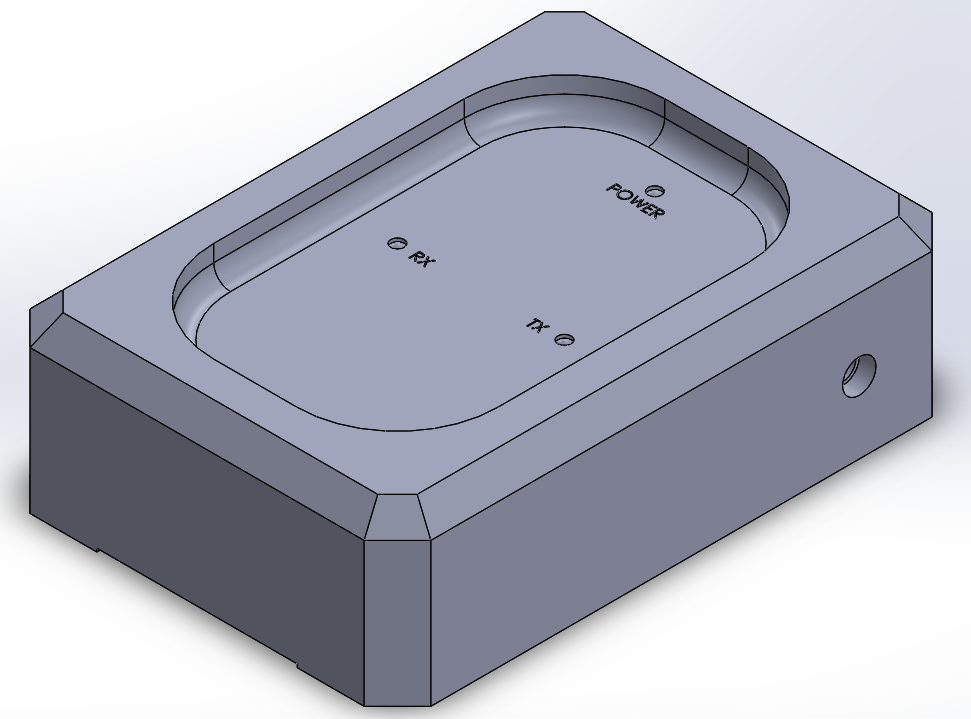
\includegraphics[scale=0.55]{./images/Beacon.png}
    \caption{Computer Aided Design representation of a Beacon}
    \label{Bcn_CAD}
\end{figure}

\pagebreak
\subsection{ID Tag Design}
The ID Tags, the part of the system being tracked by the Beacons, will be powered by a rechargeable 4.5V battery, which will be recharged slowly over time by an RF harvester (see sec. 5.2). The transceiver in the ID Tag will consist of an ESP32 module, and a DWM1000 UWB chip. The ESP32 is used in the ID tag as it has a deep sleep mode, in which the ID Tag cannot be tracked, and uses minimum power. The ID Tag will be activated in an emergency situation via capacitive touch button on the unit. If the button is pressed, and the system is not in an emergency state, the ID Tag will be put back to sleep, however if there is an emergency the ID Tag's location will then be tracked. The internal components of the ID Tag will be contained in a PLA plastic shell. There will be LEDs indicating the power state, activity, and charge level of the ID Tag. The appearance of the ID Tags can be seen in the CAD representation, Figure \ref{ID_Tag}.

medskip
\begin{figure}[H]
\centering
    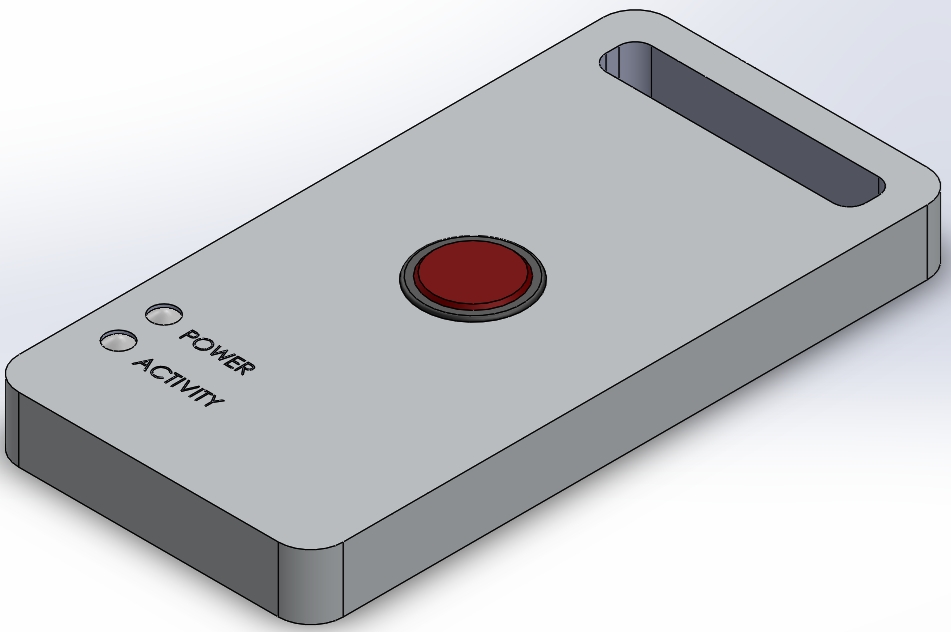
\includegraphics[scale=0.55]{./images/ID_Tag.png}
    \caption{Computer Aided Design representation of an ID Tag}
    \label{ID_Tag}
\end{figure}


\pagebreak
\subsection{DPU Design}





\pagebreak
\subsection{Hardware Design Specification}
\medskip
TRIWAVE SYSTEMS has chosen to develop the proof-of-concept prototype using 2.4 GHz Bluetooth Low Energy (BLE) modules as feasibility testing, before upgrading the system to using Ultra Wide Band (UWB) modules for further prototyping. Micro-controller Units (MCUs) will be used to control the beacons and ID tags. The requirements below detail the requirement for hardware functionality of the Akrivia Beacon system.
\medskip
\bgroup
\def\arraystretch{1.5}
\begin{table}[H]
\centering
\begin{tabular}{ | m{3cm} | m{12.5cm} |}
\hline
\textbf{REQ.HW.1 - C} & The Beacons must use ESP32 as the microcontroller unit and transceiver \\
\hline
\textbf{REQ.HW.2 - C} & The ID Tag must use ESP32 as the microcontroller unit and transceiver \\
\hline
\textbf{REQ.HW.3 - P} & ID tag broadcast duration must be at least 1 hour long upon activation\\
\hline
\textbf{REQ.HW.4 - P} & ID tag must return to deep sleep mode after broadcasting period\\
\hline
\textbf{REQ.HW.5 - P} & The Beacons must use Decawave DWM1000 UWB modules as transceivers\\
\hline
\textbf{REQ.HW.6 - P} & The Beacons must use ESP32 as the controller units\\
\hline
\textbf{REQ.HW.7 - P} & The ID tags must use Decawave DWM1000 UWB modules as transceivers\\
\hline
\textbf{REQ.HW.8 - P} & The ID tags must use ESP32 as the controller units\\
\hline
\end{tabular}
\caption{Hardware Design Specification}
\end{table}







